%-------------------------------------------------------------------------------
% LATEX TEMPLATE ARTIKEL
%-------------------------------------------------------------------------------
% Dit template is voor gebruik door studenten van de de bacheloropleiding 
% Informatica van de Universiteit van Amsterdam.
% Voor informatie over schrijfvaardigheden, zie 
%                               https://practicumav.nl/schrijven/index.html
%
%-------------------------------------------------------------------------------
%	PACKAGES EN DOCUMENT CONFIGURATIE
%-------------------------------------------------------------------------------

\documentclass{uva-inf-article}
\usepackage[english]{babel}
\usepackage{tikz}
\usepackage{pdflscape}
\usepackage{todonotes}
\usepackage{listings}
\lstset{
basicstyle=\small\ttfamily,
columns=flexible,
breaklines=true
}

\usepackage[style=authoryear-comp]{biblatex}
\addbibresource{references.bib}

%-------------------------------------------------------------------------------
%	GEGEVENS VOOR IN DE TITEL, HEADER EN FOOTER
%-------------------------------------------------------------------------------

% Geef je artikel een logische titel die de inhoud dekt.
\title{Unreal Engine Documentation}

% Vul de naam van de opdracht in zoals gegeven door de docent en het type 
% opdracht, bijvoorbeeld 'technisch rapport' of 'essay'.
% \assignment{}
% \assignmenttype{}

% Vul de volledige namen van alle auteurs in en de corresponderende UvAnetID's.
\authors{Jari Andersen}
% \uvanetids{}

% Vul de naam van je tutor, begeleider (mentor), of docent / vakcoördinator in.
% Vermeld in ieder geval de naam van diegene die het artikel nakijkt!
% \tutor{}
% \mentor{}
% \docent{}

% Vul hier de naam van je tutorgroep, werkgroep, of practicumgroep in.
% \group{SignLab, VisualisationLab}

% Vul de naam van de cursus in en de cursuscode, te vinden op o.a. DataNose.
% \course{}
% \courseid{}

% Dit is de datum die op het document komt te staan. Standaard is dat vandaag.
\date{\today}

%-------------------------------------------------------------------------------
%	VOORPAGINA 
%-------------------------------------------------------------------------------

\begin{document}
\maketitle

%-------------------------------------------------------------------------------
%	INHOUDSOPGAVE EN ABSTRACT
%-------------------------------------------------------------------------------
% Niet toevoegen bij een kort artikel, zeg minder dan 10 pagina's!

%TC:ignore
\tableofcontents
%\begin{abstract}
%\end{abstract}
%TC:endignore
\newpage
%-------------------------------------------------------------------------------
%	INHOUD
%-------------------------------------------------------------------------------
% Hanteer bij benadering IMRAD: Introduction, Method, Results, Discussion.
\section{Introduction}
Welcome to this comprehensive documentation compiled during the development journey in Unreal Engine. Throughout this document, you'll find information encompassing various aspects of development, ranging from the utilization of C++, Blueprints, and Python to defining structs for data tables. We'll also explore best practices and strategies for implementing Git, ensuring efficient collaboration and version control. Mostly, we'll touch upon bugs that we've encountered and hopefully fixed. This documentation aims to provide valuable insights and practical guidance for Unreal Engine projects.

\subsection{Live Link}
For the Live Link Pipeline documentation, go to the Unreal Live Link Pipeline documentation repository (\url{https://github.com/J-Andersen-UvA/LiveLinkPipeline-UnrealEngine}).

% \begin{landscape}
% \vspace*{\fill}
% \begin{figure}[hbt!]
%     \centering
%     \includegraphics[width=1.5\textheight]{imgs/pipeline16-2-24.png}
%     \caption{Current Live Link Pipeline. Three streams into Unreal Engine}
%     \label{fig:pipeline}
% \end{figure}
% \vspace*{\fill}
% \end{landscape}

\section{Compiling and building C++ projects}\label{CompilingAndBuilding}
When it comes to building the C++ files in Unreal we either use the IDE or Unreal Engine. Unreal Engine's compilation system comes with a functionality called Live Coding. Live coding with "hot reloading" allows developers to make changes to their C++ code while the game is running and see the changes reflected in real-time without the need to restart the game or editor. For our purposes (and because it causes many bugs), we disable the Live Coding option (see Figure \ref{fig:liveCoding} on where to disable this, and Section \ref{datatableBug} on an example bug caused by Live Coding).
\begin{figure}[hbt!]
    \centering
    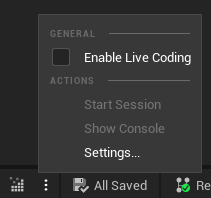
\includegraphics{imgs/livecoding.png}
    \caption{Where to disable Live Coding}
    \label{fig:liveCoding}
\end{figure}

Now we can compile in Unreal Engine or in an IDE like Visual Studio. Figure \ref{fig:vstudio} shows where to build using Visual Studio. Do make sure to follow the instructions in the following link to setup the Build tool first: \url{https://docs.unrealengine.com/4.27/en-US/ProductionPipelines/DevelopmentSetup/BuildingUnrealEngine/}. As for Unreal Engine, use the button showed in Figure \ref{fig:liveCoding}.

\begin{figure}[hbt!]
    \centering
    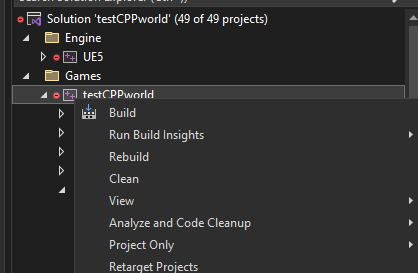
\includegraphics{imgs/buildingInVStudio.png}
    \caption{Where to build using Visual Studio}
    \label{fig:vstudio}
\end{figure}
\section{Git Version control}
We use Git for Unreal Engine to efficiently manage project versions, and to enable collaboration among team members. Git allows us to track changes to code, blueprints, and assets. By utilizing Git, Unreal Engine developers can maintain organized workflows, iterate rapidly, and coordinate effectively on complex projects.

\subsection{How to install and use Git for Unreal Engine}
Adding project to a blank repository Git:
\begin{enumerate}
    \item In the bottom right of a level screen in Unreal Engine, click revision control.
    \item Select connect to revision control.
    \item After selecting Git, add the url of your repository and initialize.
\end{enumerate}

Now you can use the same revision control button to add changes, write commits and view changes. You do however, need to push the commits by hand.
Note that sometimes some files aren't added to the Git, you'll have to fix that by adding them by hand.

\subsection{Local Plugins}
In Unreal Engine, third-party plugins play a significant role in extending functionality and enhancing project capabilities. However, unlike native plugins bundled within the Engine plugins folder, third-party plugins must be added to the project's root plugins folder due to the engine's architecture.

When we add plugins locally however, the plugins will be pushed with the rest of the project. This can cause bugs later on (see Section \ref{cppThirdPartyPluginsBug}). Especially for cloning the repository on a new machine this causes issues (follow Section \ref{cloning} for best practices on cloning a repository).

\subsection{Cloning}\label{cloning}
When cloning a repository everything usually works well. There are cases however, when cloning a repository breaks the build (for example \ref{cppThirdPartyPluginsBug}).
If we open a new project that is broken, Unreal Engine will prompt us if he can rebuild it. This works sometimes, but in cases where a local plugin prevents us to build we can do a simple trick:
\begin{itemize}
    \item Move the local plugin out of the project.
    \item Rebuild in your IDE.
    \item Open the project.
    \item Put the plugin back and rebuild.
\end{itemize}

\section{Thoughts on using C++, Python, and Blueprints}
After fighting a bit in Unreal with Python, C++, and Blueprints, we have formed thoughts on how to use and when to apply these tools. For example, C++ has nice integration with Blueprints, and it seems to be the normal way of coding in Unreal Engine. We have seen other code bases that integrate both. Therefore, we will not migrate everything to C++, but we will integrate C++ into our workflow for Unreal Engine. We can say similar things about Python. It has its own strengths, especially when coupling it with our other code that already use sockets to communicate. It is however, rather slow if we try to insert functions on every tick. With these thoughts and experiences, we decided that we will need to make careful considerations before picking our "tool" to tackle a problem.

\section{Animation editing}
Sometimes, motioncaptured animations need to be altered by hand. This section goes over how we alter animations within Unreal Engine. After importing the animations into Unreal Engine, we will the fix the animation within Unreal Engine's ``animation sequencer" (figure \ref{fig:animationsequencer}). Since the animations are baked onto the skeleton, the process of fixing the animation requires us to alter the orientation and position of the individual bones themselves. This method offers a more straightforward means of intervention compared to modifying marker data. When editing marker data, alterations become evident only after the animation is re-solved. In contrast, when addressing problematic frames and bones in this context, we can directly modify the animation. Because the alterations will be additive onto the rig, we are able to add new movements onto a bone without having to redo the entire animation. Note however, that not every animation issue can be solved with the animation sequencer. For example, extreme jitters would take too long to fix by hand.

Following is a step-by-step guide on altering animations through Unreal Engine's animations sequencer:
\begin{enumerate}
    \item Either open the animation by selecting it in the \say{level sequencer}, or open the animation and in the top \say{edit in sequencer} drop-down menu select \say{Edit With FK Control Rig}. Both sequencers are the same, but the latter doesn't require you to add the avatar to the scene by hand. For the first option make sure to bake the animation onto a FK Control Rig by right clicking the skeleton in the sequencer and selecting the \say{Edit With FK Control Rig} option.
    \item In the sequencer, add an additive section to the \say{FKControlRig} in the sequencer.
    \item Beginning with the first frame displaying odd behaviour, select the bone closest to the root displaying the abnormality or which you want to alter and create a new key-frame on the additive section in the control rig. Reposition and rotate the bone to align it with the original actor's pose. Repeat this process for all child bones. Following this, inspect the final frame of the anomalous movement. The modifications made to the initial abnormal frame will propagate throughout the animation. To restrict these alterations solely to the relevant portion, insert an additional key-frame at this specific frame and reset the additive movements. Subsequently, by adjusting the curve between these two key-frames, we can make the alterations look more natural. If the result does not appear sufficiently natural, further key-frames may be required either within or outside the altered segment to achieve a smoother transition of the adjustments. Similar to data cleaning with Shogun Post, this task is typically performed by experienced professionals, and it may require some level of practice and proficiency.
    \item Finally, when the results are adequate, right click on the skeleton in the level sequencer and select ``Bake Animation Sequence".
\end{enumerate}

\begin{figure}[hbt!]
    \centering
    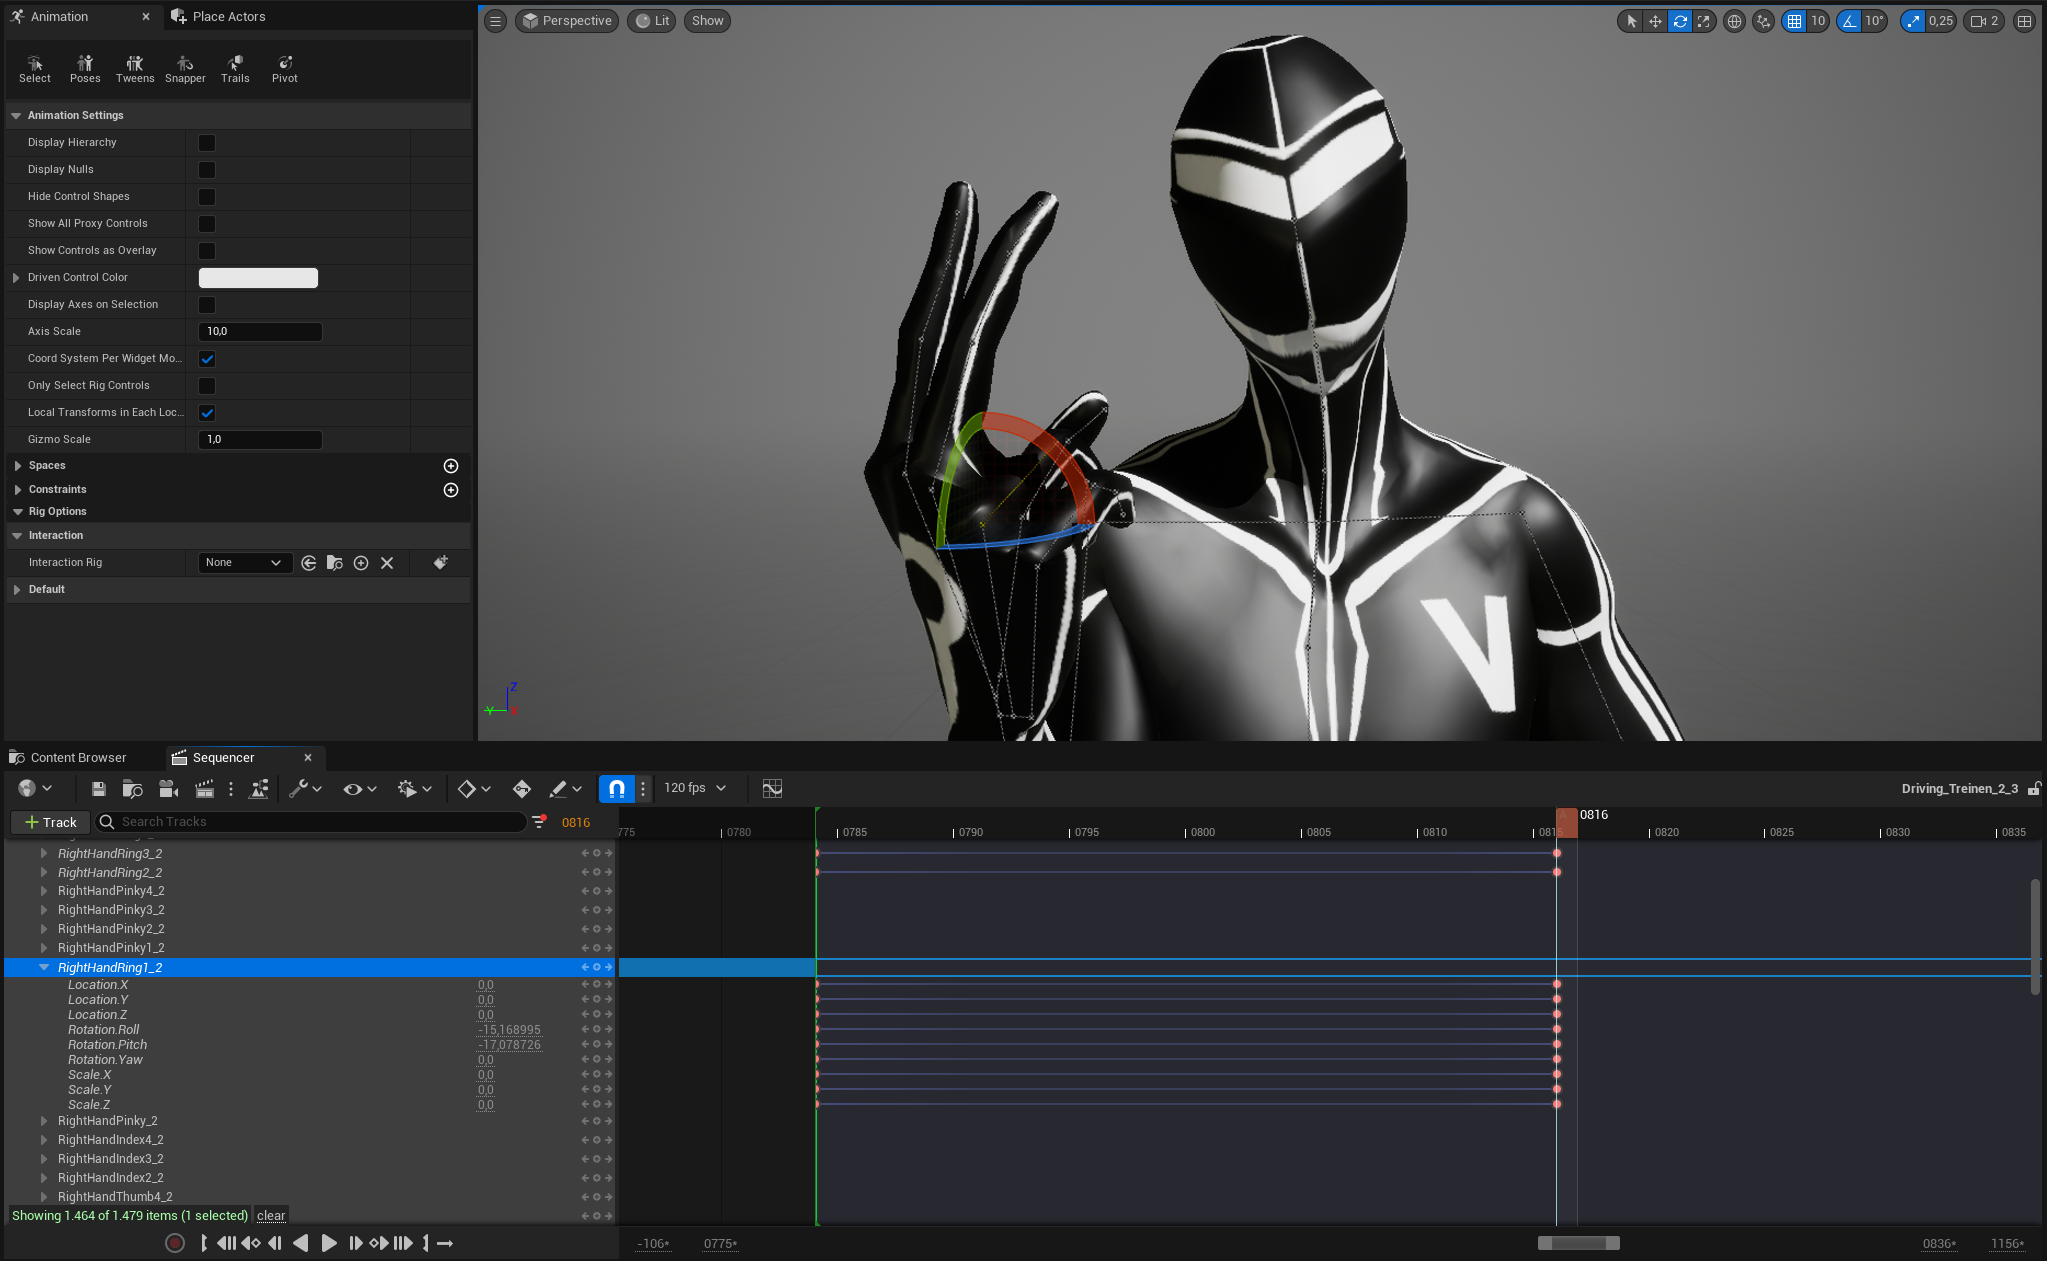
\includegraphics[width=.8\textwidth]{imgs/CleaningUpAnAnimation.png}
    \caption{The animation sequencer with an example frame being altered by using bone rotations and key-frames.}
    \label{fig:animationsequencer}
\end{figure}

\subsection{Animation bone group Blending using the sequencer}
With multiple animations we have the ability to blend between them and over each other, but what if we want to do that only for a specific bone group? Using ``Bone Grouping" or ``Animation Layering" we can force animations to play only on their relative group. Documentation wise, there is not a whole lot to go of of in Unreal Engine. Many people have made posts and videos about this, but after searching for a long while I was only able to find a single post originating from Unreal Engine 4 that goes over this topic in conjunction with the Level Sequencer. Which is exactly what we want if we want to alter animations by hand. The following link goes over this, so please have a read: \url{https://forums.unrealengine.com/t/is-it-possible-to-use-multiple-animation-slots-in-sequencer-to-layer-animations/427244/2}. In order to showcase how to do this as simple as possible and to add more difficult blendings afterwards, I have created the following step by step guide:
\begin{enumerate}
    \item Create an animation blueprint.
    \item In the Anim Slot Manager tab (can be found either in the anim graph using the window options, or in the animation itself) add an Anim Slot with the name of the parent bone which hierarchy will be grouped. In the current example, ``RightHand" is used.
    \item In the anim graph add the following:
    \begin{itemize}
        \item 2 slot ``DefaultSlot" nodes.\\Change one name to the corresponding Anim Slot to group (for example ``RightHand").
        \item A layered blend per bone node.\\In the Details tab, add a Layer with the same name as the Anim Slot (for example ``RightHand").
    \end{itemize}
    If you have applied these steps, the resulting graph will look like the one in figure \ref{fig:boneGrouping}.
    \begin{figure}[hbt!]
        \centering
        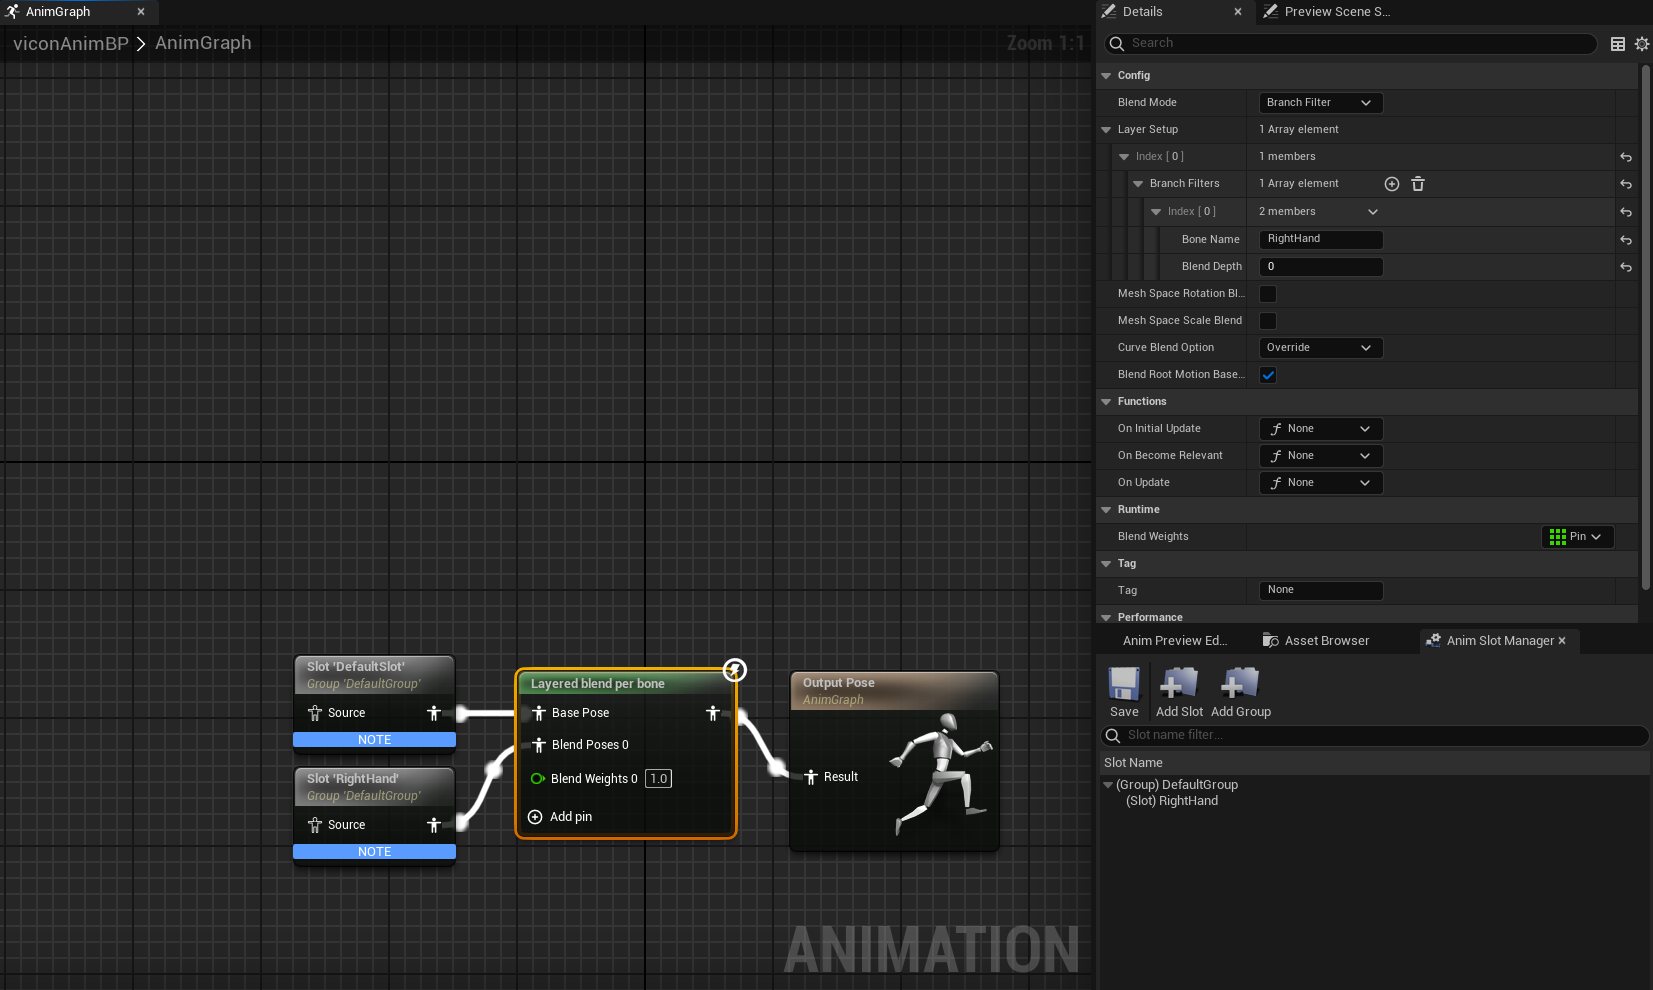
\includegraphics[width=.9\textwidth]{imgs/animgraphsimple.png}
        \caption{The simplest animation graph that applies bone grouping.}
        \label{fig:boneGrouping}
    \end{figure}
    \item Now in the normal view (world/level view) in Unreal Engine, drag the animation blueprint into the level.
    \item Open the Sequencer.
    \item Add the dragged animation blueprint to the sequencer.
    \item Add the 2 animations to be grouped (see figure \ref{fig:animSeq}).
    \begin{figure}[hbt!]
        \centering
        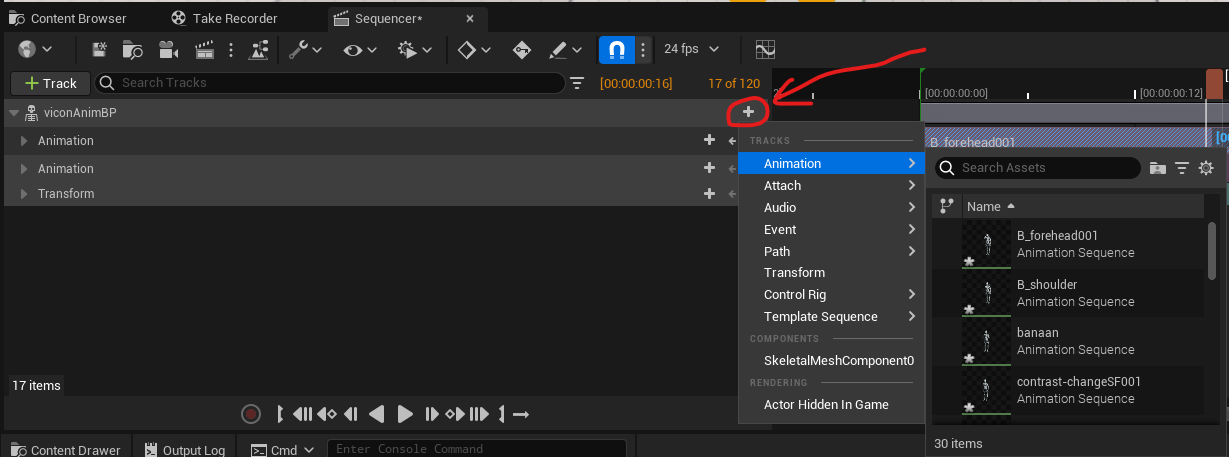
\includegraphics[width=.9\textwidth]{imgs/animationSequencer.png}
        \caption{Adding an animation to the sequencer.}
        \label{fig:animSeq}
    \end{figure}
    \item Right click the animation that we want to group, go to preferences, then type in the name of the group it should exist on (see figure \ref{fig:boneGroupPreference}).
    \begin{figure}[hbt!]
        \centering
        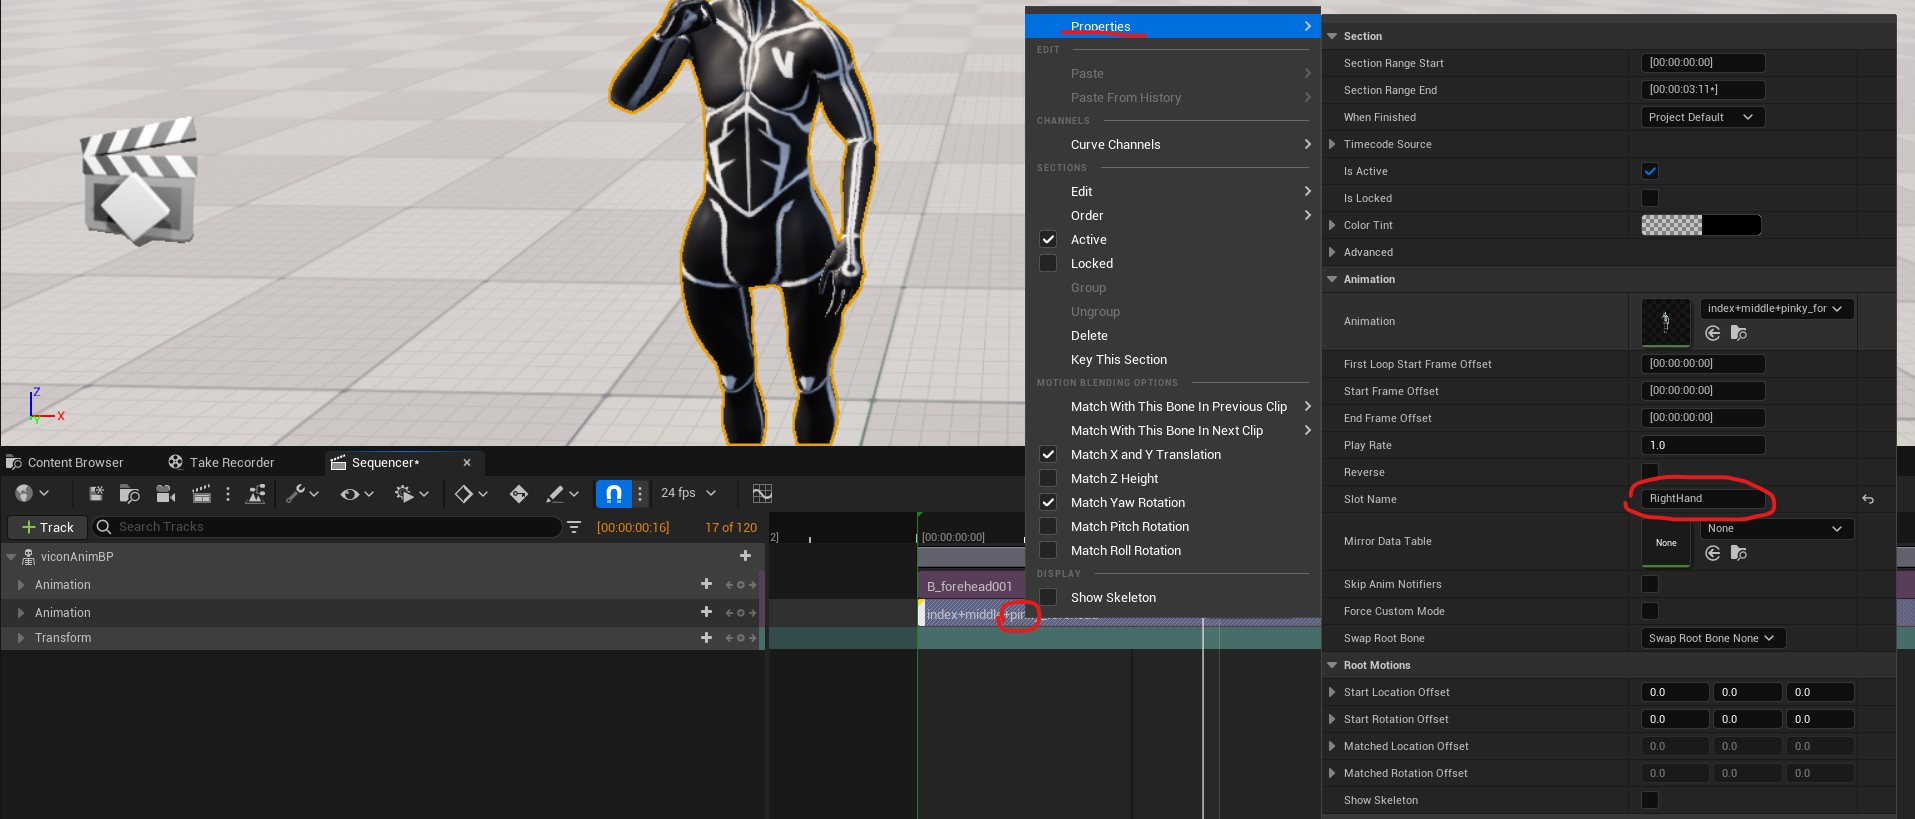
\includegraphics[width=.9\textwidth]{imgs/bonegroup.png}
        \caption{The location of the bonegroup option in the sequencer.}
        \label{fig:boneGroupPreference}
    \end{figure}
\end{enumerate}
\textit{Hint, we can define as many animation slots/bone groups as we want by adding layers to the layered blend per bone node.}

Congratulations, this is how we layer blends per bone in the level sequencer.
Now, if we want to take this further and for example blend the animation on the RightHand using 2 animations we can do the following:
\begin{enumerate}
    \item Add another animation to the sequencer.
    \item Define the animation slot in the preference menu (see figure \ref{fig:boneGroupPreference}).
    \item Tweak the weights between the 2 animations playing on the animation slot using the ``Weight" option in the level sequencer (see figure \ref{fig:weights}).
    \begin{figure}[hbt!]
        \centering
        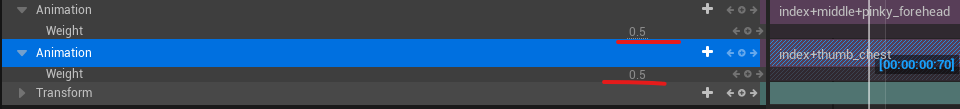
\includegraphics[width=.9\textwidth]{imgs/weights.png}
        \caption{The location of the weights option in the sequencer.}
        \label{fig:weights}
    \end{figure}
\end{enumerate}


\section{Rendering level sequences}
When we have created a level sequence that we are happy with, we have the ability to render the sequence as a video or frame sequence. To this end we use the ``Movie Render Queue" plugin.

\subsection{Blurry videos}
Make sure the camera is not set to tracking an individual avatar, the movements will create a blurry effect. Just set the camera to have no focus method.

\section{Bugs and fixes}
In the "Bugs and Fixes" section, we address challenges we encountered in Unreal Engine development hopefully along with their solutions.

\subsection{C++ projects and third party plugins}\label{cppThirdPartyPluginsBug}
Using third party plugins enables us to focus on our own development. It does come with its own challenges, however. One of which we encountered when migrating to C++ based projects. When trying to compile a project that uses third party plugins from the Engine folder that are not in the marketplace we get reference errors, example:
\begin{lstlisting}
Expecting to find a type to be declared in a module rules named 'MoCapProLiveLink' in UE5Rules, Version=0.0.0.0, Culture=neutral, PublicKeyToken=null.  This type must derive from the 'ModuleRules' type defined by Unreal Build Tool.
\end{lstlisting}
Most tips on the internet tell us to move the plugins to a project root folder called Plugins. This works, but it causes issues with the Git integration (see Section \ref{cloning} on how to fix this). One might think that we can add the module names to the build file, but in our case that did not help solve the issue.

\subsection{Datatable bug}\label{datatableBug}
Previously, we stored ``blendshape source" data, ``blendshape target" data, ``weight" data, and ``multiple blendshapes to drive" data separately within maps and arrays in blueprints. This is very redundant so we decided to move these structures to be encapsulated in a single C++ Struct. After coding this in C++ and creating a datatable out of this in Unreal Engine, we populated it with data (an example of a single entry can be seen in Figure \ref{fig:blendshapeStructExample}).

\begin{figure}[hbt!]
    \centering
    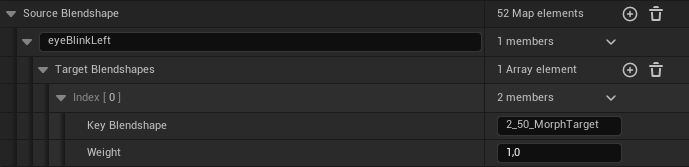
\includegraphics[width=\textwidth]{imgs/singleBlendshapeData.png}
    \caption{An example source blendshape that drives a single target blendshape with a weight of 1.}
    \label{fig:blendshapeStructExample}
\end{figure}

This worked very well until we closed the editor, re-opened it and tried to view the datatable again. We get prompted by Unreal with an Error message. Pressing "Yes" at error message will open the asset without any of the struct information. Where did our data go? After a lot of fighting, we broke the entire project again and we had to rebuild through our IDE. Somehow that fixed the issue for the datatable as wel. Later into development the table was not useable in a blueprint, however. After further inspection we noticed that the ``RowStruct" of the datatable changed to something prepended with ``LIVECODE". Therefore we concluded that the entire problem was caused by the hotloading functionality of Unreal's compilation system. Disabling this functionality fixed the problem (more on best practices for compiling in Section \ref{CompilingAndBuilding}).

\subsection{Exporting/importing Datatables}
When exporting a datatable, you might be tempted to export it the same way you would export any other asset. That doesn't work however. Simply export it as csv or json in order to import it in a new project. In the new project, create a new datatable, open it, and use the reimport button to import the csv or json.

%-------------------------------------------------------------------------------
%	REFERENTIES
%-------------------------------------------------------------------------------

\printbibliography

%-------------------------------------------------------------------------------
%	BIJLAGEN 
%-------------------------------------------------------------------------------

%TC:ignore
% \appendix 
% \section{Bijlage {\LaTeX} code}
% Bijgevoegd zijn de \textattachfile{main.tex}{code} en 
% \textattachfile{references.bib}{bibliografie}.
%TC:endignore

%-------------------------------------------------------------------------------
\end{document}